\begin{figure}[!htb]
    \centering
    \begin{subfigure}{0.35\textwidth}
        \centering
        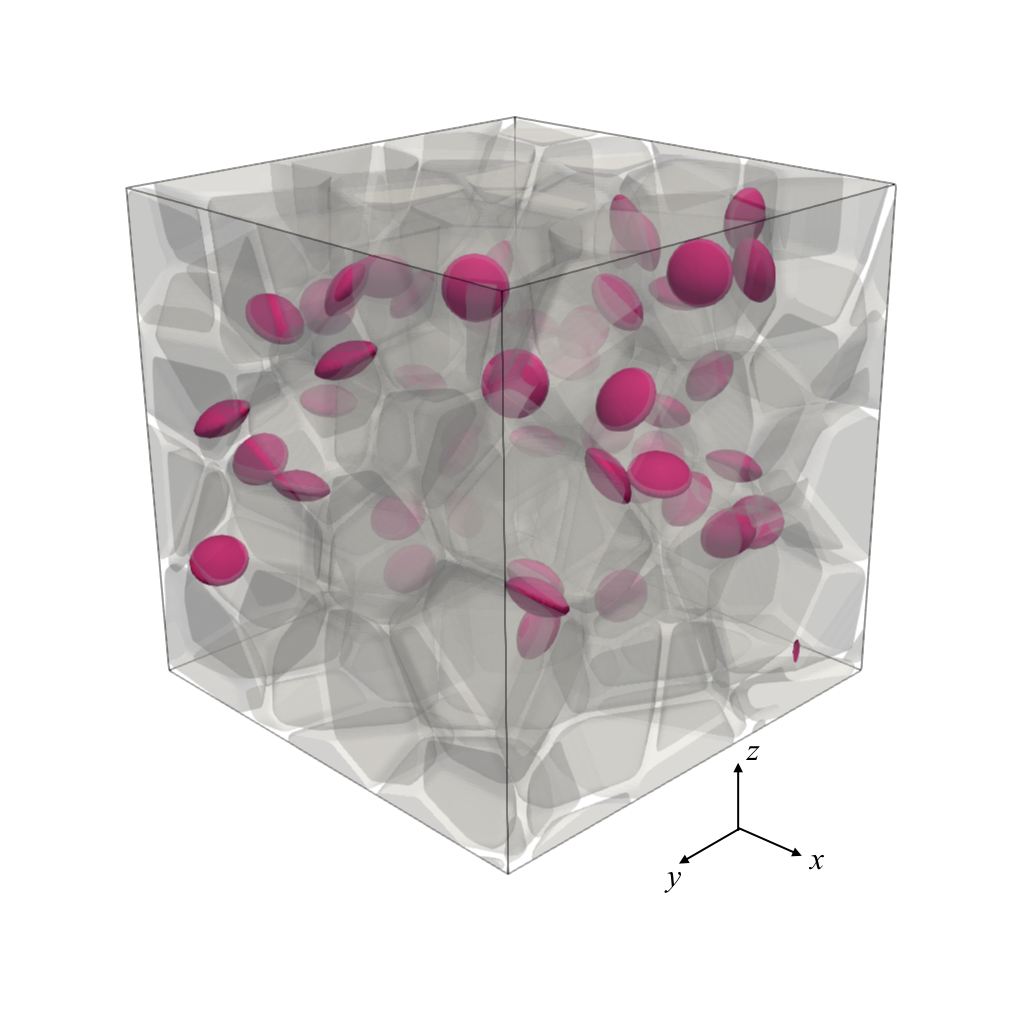
\includegraphics[width=\textwidth]{past/figures/b50_ini_new.png}
    \end{subfigure}
    \begin{subfigure}{0.35\textwidth}
        \centering
        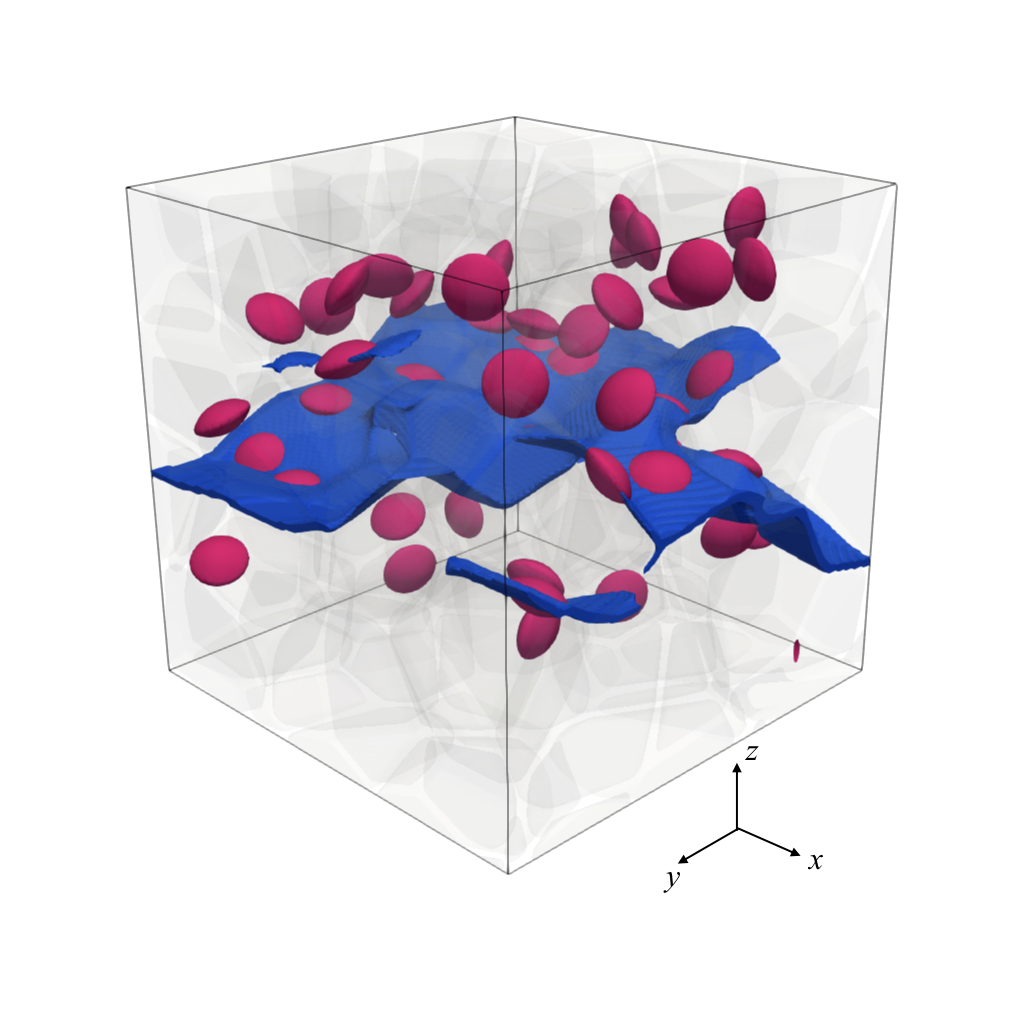
\includegraphics[width=\textwidth]{past/figures/b50_end.png}
    \end{subfigure}

    \vspace{-0.1in}
    \begin{subfigure}{0.35\textwidth}
        \centering
        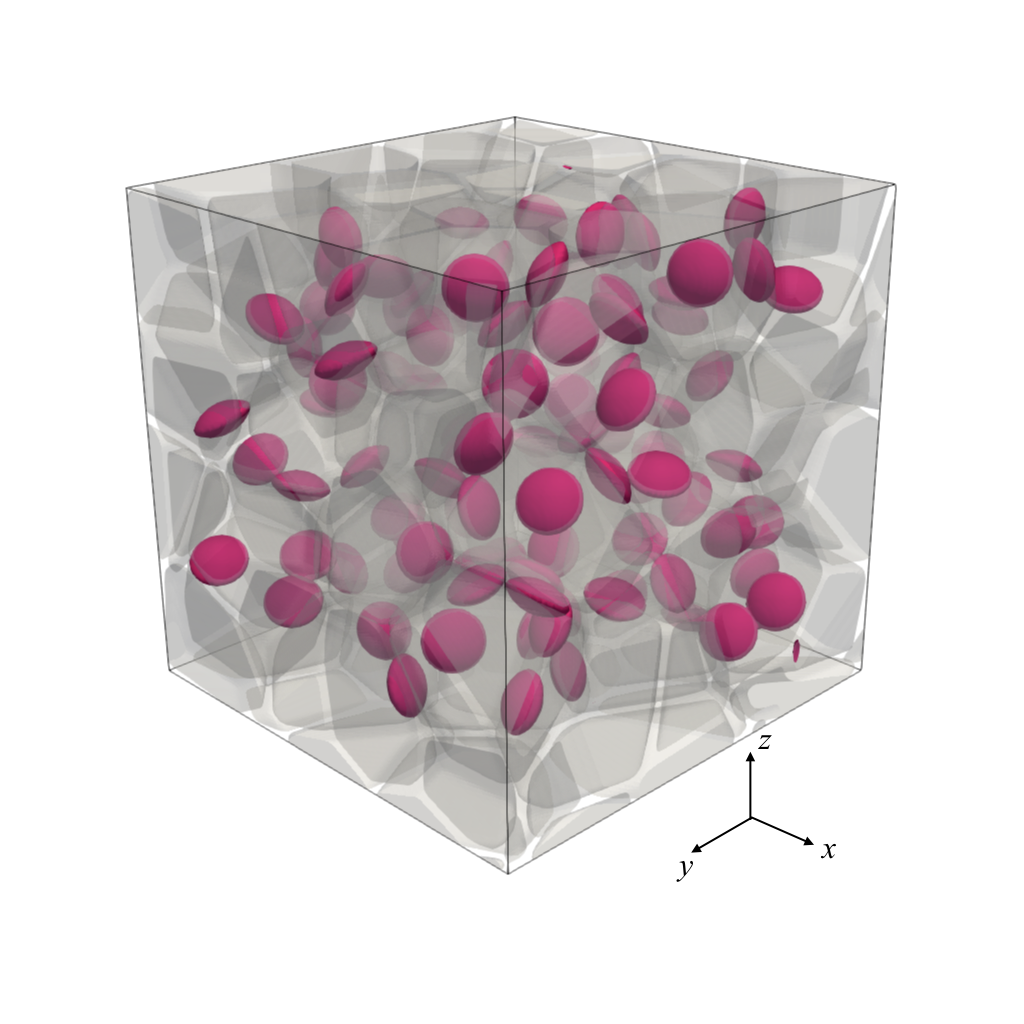
\includegraphics[width=\textwidth]{past/figures/b100_ini_new.png}
    \end{subfigure}
    \begin{subfigure}{0.35\textwidth}
        \centering
        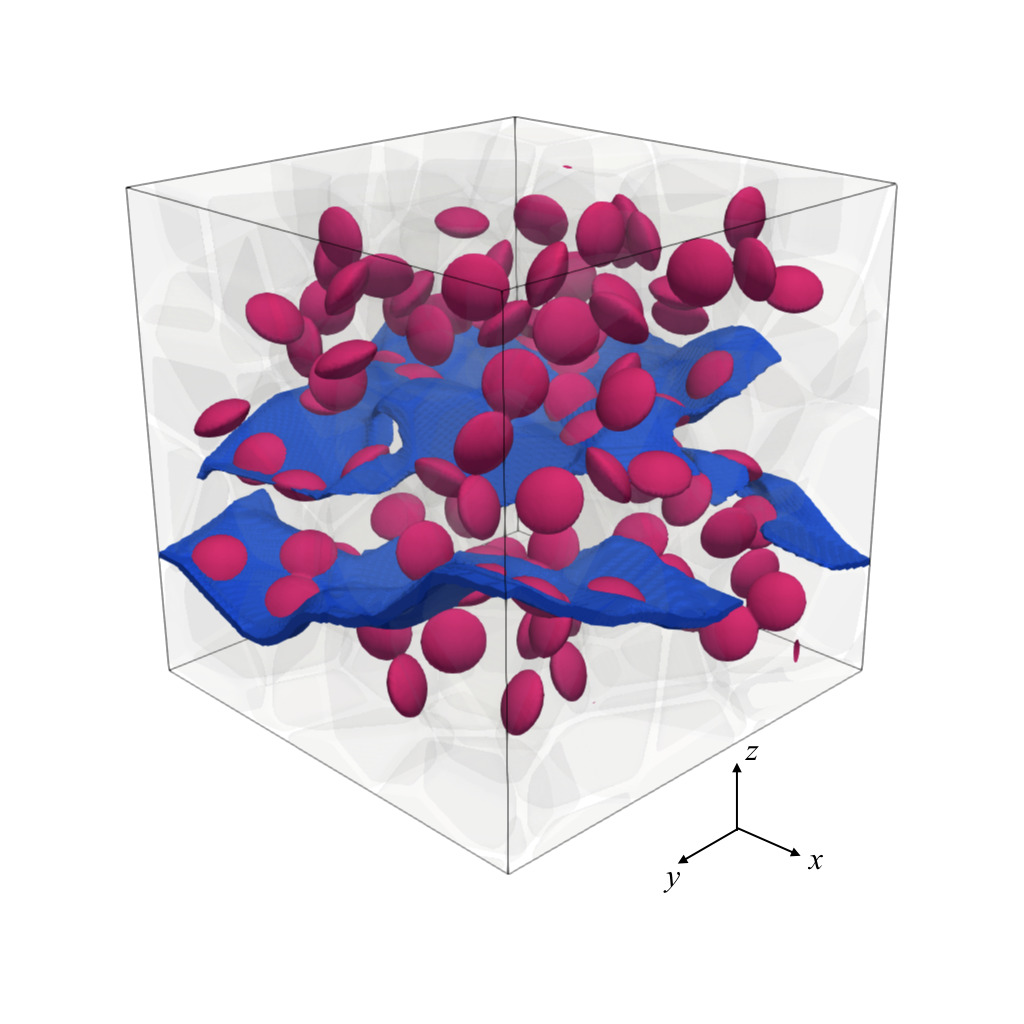
\includegraphics[width=\textwidth]{past/figures/b100_end.png}
    \end{subfigure}

    \vspace{-0.1in}
    \begin{subfigure}{0.35\textwidth}
        \centering
        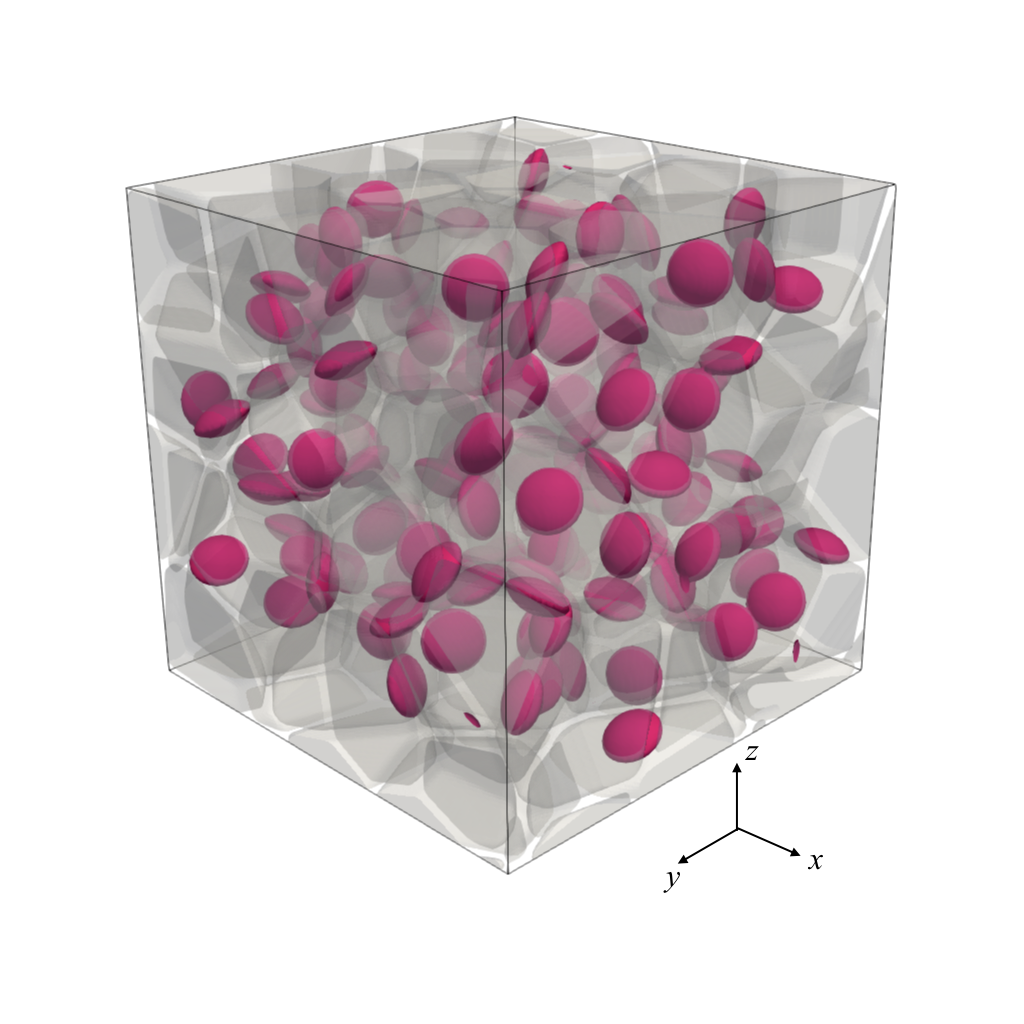
\includegraphics[width=\textwidth]{past/figures/b150_ini_new.png}
    \end{subfigure}
    \begin{subfigure}{0.35\textwidth}
        \centering
        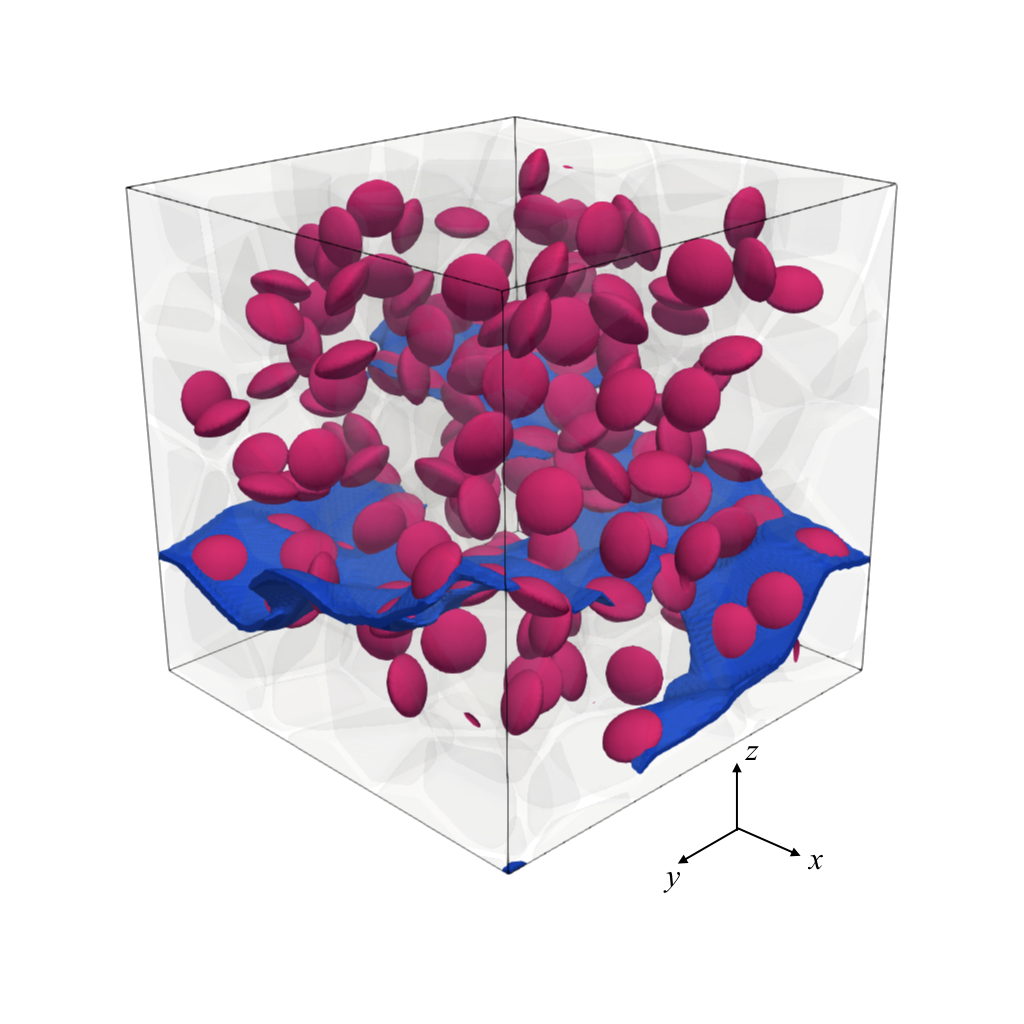
\includegraphics[width=\textwidth]{past/figures/b150_end.png}
    \end{subfigure}

    \begin{tikzpicture}
        \begin{axis}[
            width=\textwidth,
            height=0.6\textwidth,
            ticks=none,
            xlabel=Strain,ylabel=Stress,
            xmin=0,
            xmax=0.0025,
            ymin=0,
            ymax=700,
            every axis plot/.append style={line width=1pt}
        ]
            \addplot +[mark=none,color=black,solid] table[x expr=\thisrowno{2}/40,y=ave_stress_top] {past/data/b50_out.csv};
            \addplot +[mark=none,color=black,dashed] table[x expr=\thisrowno{2}/40,y=ave_stress_top] {past/data/b100_out.csv};
            \addplot +[mark=none,color=black,dotted] table[x expr=\thisrowno{2}/40,y=ave_stress_top] {past/data/b150_out.csv};
        \end{axis}
    \end{tikzpicture}
\end{figure}
